%%%%%%%%%%%%%%%%%%%%%%%%%%%%%%%%%%%%%%%%%%%%%%%%%%%%%%%%%%%%%%%%%%%%%%%%%%%%%%%%%%%%%%%%%%%%%%%%%
%
% Document:     DM Support Prd.  product tree
%
%%%%%%%%%%%%%%%%%%%%%%%%%%%%%%%%%%%%%%%%%%%%%%%%%%%%%%%%%%%%%%%%%%%%%%%%%%%%%%
\documentclass{article}
\usepackage{times,layouts}
\usepackage{tikz,hyperref,amsmath}
\usetikzlibrary{positioning,arrows,shapes,decorations.shapes,shapes.arrows}
\usetikzlibrary{backgrounds,calc}
\usepackage[paperwidth=26.0cm,paperheight=8.3cm,
left=-2mm,top=3mm,bottom=0mm,right=0mm,
noheadfoot,marginparwidth=0pt,includemp=false,
textwidth=30cm,textheight=50mm]{geometry}
\newcommand\showpage{%
\setlayoutscale{0.5}\setlabelfont{\tiny}\printheadingsfalse\printparametersfalse
\currentpage\pagedesign}
\hypersetup{pdftitle={DM products }, pdfsubject={Diagram illustrating the
                products in LSST DM }, pdfauthor={Autogenerated from MD}}
\tikzstyle{tbox}=[rectangle,text centered, text width=30mm]
\tikzstyle{wbbox}=[rectangle, rounded corners=3pt, draw=black, top color=blue!50!white,
                    bottom color=white, very thick, minimum height=12mm, inner sep=2pt,
                    text centered, text width=30mm]
\tikzstyle{pbox}=[rectangle, rounded corners=3pt, draw=black, top
 color=yellow!50!white, bottom color=white, very thick,
 minimum height=35pt, inner sep=2pt, text centered, text width=35mm]
\tikzstyle{pline}=[-, thick]
\begin{document}
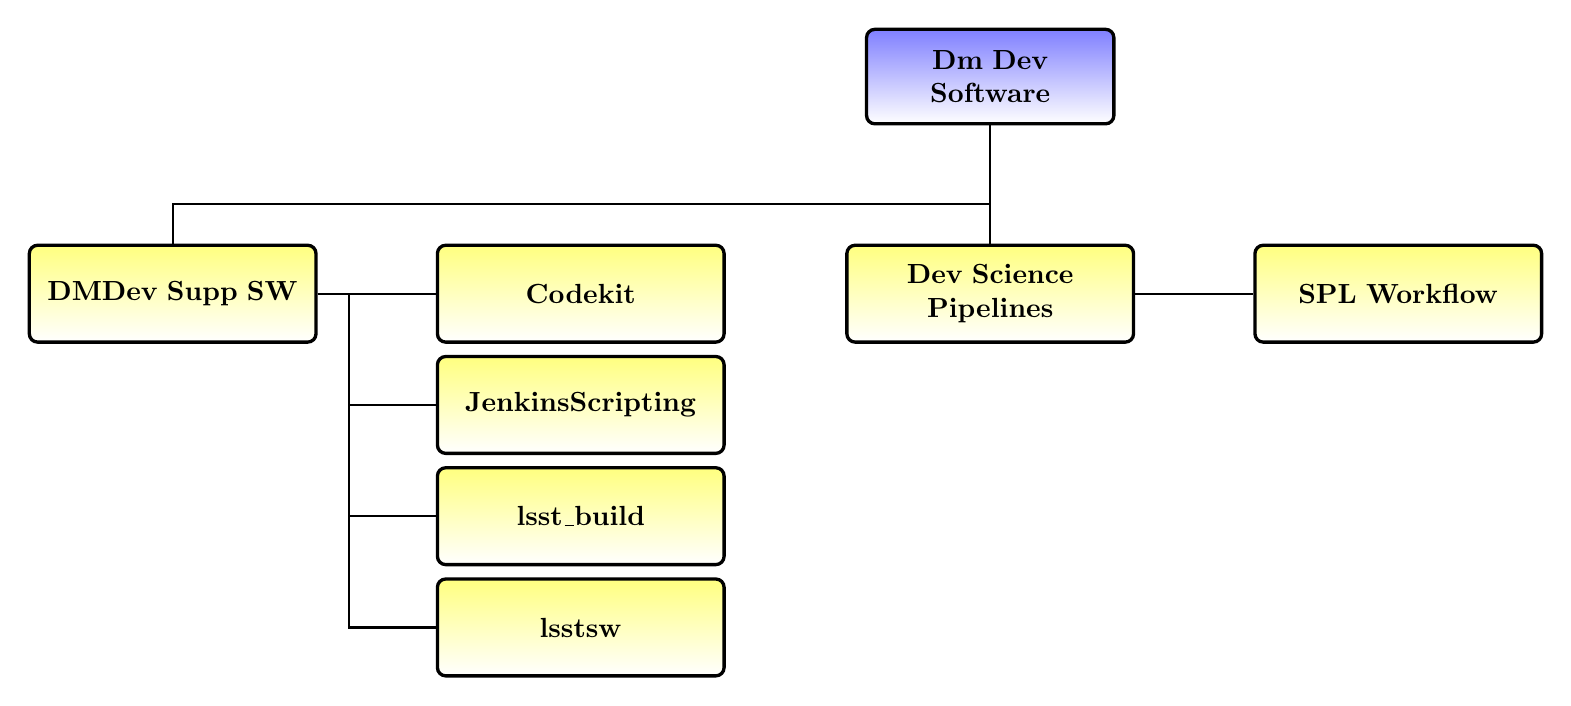
\begin{tikzpicture}[node distance=0mm]


\node (DMDSS) [pbox, 
] {\textbf{DMDev Supp SW
} };
\node (CDKT) [pbox,right=15mm of DMDSS] {\textbf{Codekit
} };
 \draw[pline] (DMDSS.east) -| ++(0.4,0) |- (CDKT.west); 
\node (JSCR) [pbox,below=4pt of CDKT] {\textbf{JenkinsScripting
} };
 \draw[pline] (DMDSS.east) -| ++(0.4,0) |- (JSCR.west); 
\node (LBLD) [pbox,below=4pt of JSCR] {\textbf{lsst\_build
} };
 \draw[pline] (DMDSS.east) -| ++(0.4,0) |- (LBLD.west); 
\node (LSSTSW) [pbox,below=4pt of LBLD] {\textbf{lsstsw
} };
 \draw[pline] (DMDSS.east) -| ++(0.4,0) |- (LSSTSW.west); 
\node (DSPLSW) [pbox, 
right=6.7cm of DMDSS] {\textbf{Dev Science Pipelines
} };
\node (SPLWF) [pbox,right=15mm of DSPLSW] {\textbf{SPL Workflow
} };
 \draw[pline] (DSPLSW.east) -| ++(0.4,0) |- (SPLWF.west); 
\node (DMDSW) [wbbox, above=15mm of DSPLSW]{\textbf{Dm Dev Software
}};
 \draw[pline]   (DMDSS.north) -- ++(0.0,0.5) -| (DMDSW.south) ; 
 \draw[pline]   (DSPLSW.north) -- ++(0.0,0.5) -| (DMDSW.south) ; 

\end{tikzpicture}
\end{document}
